\begin{pastexam}[label={px:nchu-113-dsa-07}]{中興資工所甲組 113 學年度 選擇題第 7 題}
（單選；每題 2 分，答錯倒扣 0.5 分）

\textit{The next three questions apply to the following tree T containing 14 nodes, where each node
corresponds to an integer:}

\begin{center}
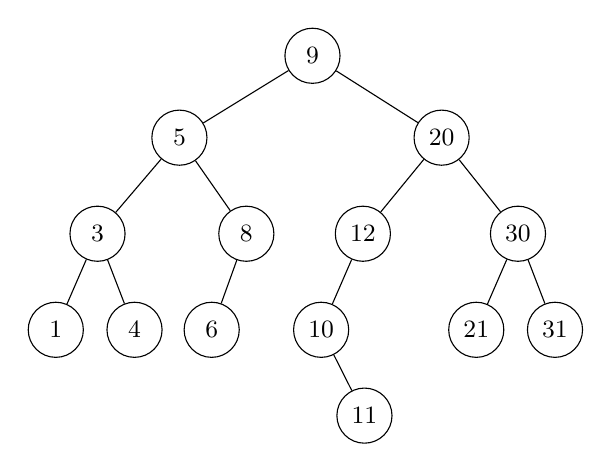
\begin{tikzpicture}[v/.style={circle,draw,minimum size=7mm,inner sep=1pt,font=\small}]
\node[v] (n9)  at (3.26,3.48) {9};
\node[v] (n5)  at (1.57,2.44) {5};
\node[v] (n20) at (4.90,2.44) {20};
\node[v] (n3)  at (0.53,1.22) {3};
\node[v] (n8)  at (2.42,1.22) {8};
\node[v] (n12) at (3.90,1.22) {12};
\node[v] (n30) at (5.87,1.22) {30};
\node[v] (n1)  at (0.00,0) {1};
\node[v] (n4)  at (1.00,0) {4};
\node[v] (n6)  at (1.98,0) {6};
\node[v] (n10) at (3.37,0) {10};
\node[v] (n21) at (5.34,0) {21};
\node[v] (n31) at (6.34,0) {31};
\node[v] (n11) at (3.92,-1.09) {11};
\draw (n9)--(n5) (n9)--(n20) (n5)--(n3) (n5)--(n8) (n20)--(n12) (n20)--(n30)
  (n3)--(n1) (n3)--(n4) (n8)--(n6) (n12)--(n10) (n30)--(n21) (n30)--(n31) (n10)--(n11);
\end{tikzpicture}
\end{center}

What is the sum of the order of 7\textsuperscript{th}, 9\textsuperscript{th}, 13\textsuperscript{th} node if we apply the \textbf{in-order} traversal of \textit{T}?

(A)~39 \qquad (B)~50 \qquad (C)~53 \qquad (D)~51 \qquad (E)~None of the above.
\end{pastexam}

\begin{pastsoln}
答案是 (B)。

$T$ 的結構：根 $9$，左子節點 $5$、右子節點 $20$；$5$ 的左右是 $3$、$8$，$3$ 的左右是 $1$、$4$，$8$ 只有左子節點 $6$；
$20$ 的左右是 $12$、$30$，$12$ 只有左子節點 $10$，$10$ 只有右子節點 $11$，$30$ 的左右是 $21$、$31$。 （圖上 $6$
在 $8$ 的左下、$10$ 在 $12$ 的左下、$11$ 在 $10$ 的右下。） 題目的「order of $k$th node」指走訪順序中第 $k$ 個
節點的值。

$T$ 正好是一棵二元搜尋樹（每個節點都大於左子樹、小於右子樹），所以中序（左、根、右）就是由小到大：
\begin{center}
\small
\begin{tabular}{l*{14}{c}}
\toprule
位置 & 1 & 2 & 3 & 4 & 5 & 6 & 7 & 8 & 9 & 10 & 11 & 12 & 13 & 14 \\
\midrule
節點 & 1 & 3 & 4 & 5 & 6 & 8 & \textbf{9} & 10 & \textbf{11} & 12 & 20 & 21 & \textbf{30} & 31 \\
\bottomrule
\end{tabular}
\end{center}
第 7、9、13 個是 $9$、$11$、$30$，和是 $9 + 11 + 30 = 50$，選 (B)。 照左、根、右逐點走一次也得到同樣的
順序：$8$ 只有左子節點，所以 $6$ 在 $8$ 前面；$10$ 只有右子節點，所以 $10$ 在 $11$ 前面。
\end{pastsoln}
